\documentclass[main.tex]{subfiles}

\begin{document}
\section{Teori}
\subsection{Z80}
Z80 är en processor från 1976 tillverkad av Zilog. Den är fullt kompatibel med
Intel 8080 men har även extra instruktioner och register. Nedan följer en kort
beskrivning till vissa aspekt av processorn. Mer detaljerad information om
processorn kan hittas i Zilog:s användarmanual.\cite{z80um}

\begin{figure}
    \center
    \includegraphics[width=0.9\textwidth]{z80arch.eps}
    \caption{Ett approximativt blockschema av Z80-processorn. Av {\it
    Appaloosa}, CC BY-SA 3.0.}
\end{figure}

\paragraph{Register}
    Processorn har åtta 8-bitars register och och tre 16-bitars register.
    Register med en bokstav är 8 bitar och register med två bokstäver är 16
    bitar. Programmerare kan direkt komma åt och använda de flesta av dessa för
    allmänna behov. Vissa register har dock speciella instruktioner och
    specifika användningsområden. Par av 8-bitars register kan även användas
    som 16-bitars register av vissa instruktioner som bland annat \mono{push
    BC} och \mono{add HL, DE}. Det finns även ett par av register som
    programmeraren inte har tillgång till. Dessa är \mono{W} och \mono{Z} och
    används endast internt av processorn.
\begin{labeling}{indent}
\item[\mono{A}]
    Kallas även för ``ackumulator'', det är det primära registret för
    aritmetiska operationer och för att nå minnet. Registret är direkt kopplat
    till ALU:n och kan användas som indata för matematiska instruktioner som
    till exempel \mono{add a, b}.
\item[\mono{B}]
    Vissa instruktioner använder \mono{B} som räknare.
\item[\mono{C}]
    Används bland annat för att lagra lagra portnumret vid en \mono{in}- eller
    \mono{ut}-instruktion. Tillsammans med B kan
\item[\mono{D}, \mono{E}]
    Används bland annat parvis för att lagra minnesadresser. Till exempel som
    destinationsadress för \mono{ldir} som flyttar ett block i minnet.
\item[\mono{F}]
    Registret som lagrar flaggorna. Vilken bit som representerar vad kan visas
    i figur \ref{fig:flags}. Under en ALU-instruktion laddas \mono{F} med
    flaggorna. Det finns inga flyttnings- eller räkneinstruktioner såsom
    \mono{ld} eller \mono{sub} som använder \mono{F}. \mono{F} ändras endast
    indirekt via ALU:n. Det går dock att läsa och skriva till \mono{F} via
    stacken med \mono{push af} och \mono{pop af}.
\item[\mono{H}, \mono{L}]
    Register som ofta parvis lagrar en minnesadress. Många instruktioner
    använder HL för att referera till en plats i minnet.  Dessa register kan
    även byta plats med \mono{DE} med \mono{ex de, hl}-instruktionen.
\item[\mono{IX}, \mono{IY}]
    Dessa används på liknande sätt som \mono{HL} men istället för att använda
    adressen som registret pekar på används relativ adressering. Ett exempel är
    instruktionen \mono{and (ix+d)} som utför \mono{and} på värdet som ligger
    \mono{d} platser efter adressen som \mono{IX} pekar på.
\item[\mono{SP}]
    Stackpekaren, pekar på den nuvarande adressen till toppen av stacken.
    Speciella instruktioner som \mono{push}, \mono{pop} och \mono{call}
    modifierar \mono{SP} medan programmerarens förmåga att direkt modifiera
    \mono{SP} är begränsad.
\item[\mono{I}]
    \mono{I} används i samband med avbrottshantering. Lagrar den översta byte:n
    av adressen till en hoppadress för avbrottsläge 2.
\item[\mono{R}]
    Register för memory refresh. Z80:n har inbyggd refresh-hantering för
    dynamiska minnen.
\item[\mono{PC}]
    Instruktionspekaren, lagrar minnesplatsen som processorn ska hämta nästa
    instruktion ifrån. Inga funktioner kan ändra PC direkt, endast indirekt med
    hoppinstruktioner.
    % jp **, jp (hl) fungerar precis som ld pc,**; ld pc,hl skulle göra.
    % så man kan ju typ ändra pc direkt, kanske omformulera/förtydliga
\end{labeling}

\paragraph{Flaggor}

\begin{figure}
    \center
    \begin{tabular}{|l|c|c|c|c|c|c|c|c|}
        \hline
        bit     & 7 & 6 & 5 & 4 & 3 & 2 & 1 & 0 \\ \hline
        flagga  & S & Z & Y & H & X & P & N & C \\ \hline
    \end{tabular}
    \caption{Flaggornas uppsättning i \mono{F}-registret.}
    \label{fig:flags}
\end{figure}

\begin{itemize}
    \item \mono{C} carry - Används framförallt för att indikera minnessiffra
        vid addition och lån vid subtraktion. Vid aritmetisk operation är det
        en kopia av den bit 8. För vissa rotationsinstruktioner lagras en av
        operandens kanter i carry-flaggan.
    \item \mono{N} subtract - Indikerar att instruktionen är en subtraktion.
        Används endast av \mono{daa} för att korrigera resultatet till BCD.
    \item \mono{P} parity/overflow - \mono{P} visar om en aritmetisk overflow
        har inträffat för aritmetiska instruktioner. För bitinstruktioner som
        bland annat \mono{xor} visar \mono{P} om resultatet har paritet (jämnt
        antal nollor). \mono{P} används även för att indikera om \mono{BC} är
        noll vid blockinstruktioner som \mono{ldir}. Flaggan sätts även till
        värdet av \mono{IFF} vid exekveringen av \mono{ld a, i} och \mono{ld a,
        r}.
    \item \mono{X} - Odokumenterad, har ingen funktion, kallas även för
        \mono{f3}. Generellt så är det en kopia av bit 3 av resultatet.
    \item \mono{H} half-carry - Indikerar carry för resultatet av de första
        fyra bitarna. Z80:n har en 4-bitars ALU så den här flaggan kommer
        därför naturligt.
    \item \mono{Y} - Odokumenterad, som \mono{X} men kopia av bit 5.
    \item \mono{S} sign - Indikerar om resultatet är negativt om tolkat som ett
        tvåkomplementstal. Det är en kopia av bit 7 i resultatet.
    \item \mono{Z} zero - Indikerar att resultatet är noll.
\end{itemize}

\paragraph{Externa bussar}
Z80:n har en 8-bitars databuss och en 16-bitars adressbuss. Processorn både
skriver och läser till och från databussen men skriver endast till
adressbussen. Det finns också en så kallad kontrollbuss som består av flera in-
och utsignaler. Insignalerna består av \mono{INT}, \mono{NMI}, \mono{RESET},
\mono{BUSREQ} och \mono{WAIT}. \mono{INT} används för att signalera ett
avbrott, \mono{NMI} för ett {\it nonmaskable interrupt}. \mono{WAIT} används
vid minnes- eller IO-operationer för att indikera att indatan ännu inte är
redo. \mono{BUSREQ} signalerar till processorn att en enhet vill använda så att
processorn sätter databussen och adressbussen till högimpedans. Utsignalerna
består av \mono{HALT}, \mono{M1}, \mono{IORQ}, \mono{MREQ}, \mono{RD},
\mono{WR}, \mono{RFSH}, \mono{BUSACK}. \mono{HALT} är aktiv när processorn är i
halt-läge. \mono{M1} är aktiv när processorn är i maskincykel ett. Om
processorn hämtar från minnet när \mono{M1} är aktiv innebär det att processorn
hämtar en instruktion. Med hjälp av \mono{RD} och \mono{WR} signalerar
processorn att den ska läsa eller skriva. Samtidigt signalerar processorn om
den vill läsa/skriva till minnet eller till en IO-enhet med hjälp av
\mono{IORQ} och \mono{MREQ}-signalerna. \mono{IORQ} med \mono{M1} kan även
indikera att processorn är redo att läsa från databussen under ett avbrott.
\mono{RFSH} används för att skicka refresh-signaler till ett dynamiskt minne.
\mono{BUSACK} går aktiv när processorn har lagt hög impedans på bussarna efter
en \mono{BUSREQ}-signal.

\paragraph{IO}
Z80-processorn har ett system av portar för att hantera in- och utdata till
andra enheter utöver minne. När ett program vill skicka data till en enhet
används en av \mono{OUT}-instruktionerna. Då placeras portnumret på
adressbussens lägre åtta bitar och utdatan läggs på databussen av processorn så
att IO-enheten som korresponderar till den porten tar emot den. Under en
\mono{IN}-instruktion placerar processorn porten på adressbussen men
korresponderande IO-enhet placerar sin data på databussen. För att det här
systemet ska fungera måste en dedikerad enhet utanför processorn hantera
muxning av data till och från rätt enhet utifrån porten på adressbussen.

\paragraph{Avbrott}
Vid början av exekveringen av varje instruktion kontrollerar processorn om
\mono{INT} eller \mono{NMI} är aktiva. Vid en aktiv \mono{INT}-signal reagerar
processorn på olika sätt beroende på vilket läge som är inställt av
programmeraren. Processorn har tre olika avbrottslägen som kan väljas med
instruktionerna \mono{im 0}, \mono{im 1} och \mono{im 2}. Det finns även två
D-vippor \mono{IFF1} och \mono{IFF2}. Processorn svarar endast på en
\mono{INT}-signal om \mono{IFF1} är 1. Programmeraren kan välja dess värde med
instruktionerna \mono{ei} och \mono{di}. \mono{IFF2} används för att lagra
\mono{IFF1}:s värde under en {\it nonmaskable interrupt}.

Vid avbrott under läge 0 hämtar processorn en 8-bitars instruktion från
databussen och exekverar den. Instruktionen kan till exempel vara en \mono{rst
28h} som direkt hoppar till adress \mono{0x0028}. Processorn lägger även
\mono{PC} på stacken så att processorn kan återvända till programmet när
avbrottsrutinen är färdig och kör \mono{reti}. Under avbrottet återställs även
\mono{IFF1} och \mono{IFF2} så att ett nytt avbrott inte kan ske under
avbrottsrutinen.  Avbrottsrutinen måste själv sätta igång avbrott igen med
\mono{ei}. För att ett avbrott inte ska kunna ske mellan \mono{ei} och
\mono{reti}-instruktionerna så kommer processorn inte acceptera avbrott förrän
en instruktion efter att \mono{ei} har använts.

Vid läge 1 hoppar processorn alltid till adress 0x38. Detta motsvarar en
\mono{rst 38h}-instruktion.

Vid läge 2 kommer processorn att hämta de lägre åtta bitarna av en adress från
databussen. I \mono{I}-registret ligger de åtta högre bitarna av adressen till
en hoppadress som ligger i minnet. Processorn kommer hämta hoppadressen från
denna adress minnet och lägga den i PC så att ett hopp utförs.

Vid en \mono{NMI}-signal kommer processorn reagera precis som under läge 1 men
att den hoppar till adress 0x66 istället för 0x38. Dessa avbrott sker oavsett
om \mono{IFF1} är 1 eller 0. Vid sådana avbrott återställs \mono{IFF1} precis
som innan för att förhindra avbrott men \mono{IFF2} antar nu värdet av
\mono{IFF1}. På så sätt kan föregående värdet av \mono{IFF1} återställas när
avbrottsrutinen är färdig och exekverar \mono{retn}-instruktionen.

\newpage
\subsection{TI-83p}

\begin{wrapfigure}{r}{0.4\textwidth}
    \centering
    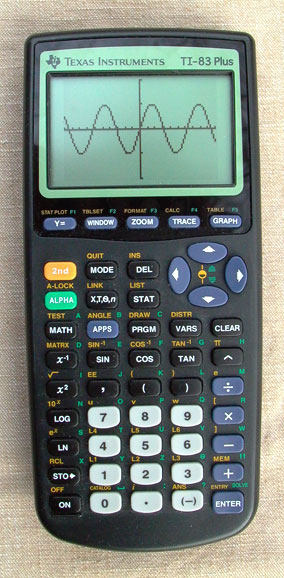
\includegraphics[width=0.4\textwidth, bb=0 0 284 578]{img/ti83p.jpg}
    \caption{En TI83p-miniräknare från Texas Instruments. Bild av
    Westernelectric555, public domain.}
    \label{fig:ti83p}
\end{wrapfigure}

Miniräknaren TI-83p är en grafritande miniräknare tillverkad av Texas
Instruments. Miniräknaren använder en Z80 processor klockad till 6MHz, en 96x64
monokrom LCD-skärm. TI-miniräknarna har en inbyggd {\it application specific
integrated circuit} (ASIC) som bland annat muxar data mellan processorn och
portarna. TI83p:an använder sig av en T6A04 LCD kontroller. Detaljerad
information om dess funktionalitet finns i dess datablad\cite{t6a04}. Andra
delar av TI83p:ans ASIC är odokumenterade men den innehåller bland annat
hårdvarutimers, avbrottshanterare, tangentbordskontroller, minnesmappning och
minnesskydd.

TI83p använder sig inte av alla Z80:ns funktioner. Bland annat används inte
{\it nonmaskable interrupts} eftersom ASIC:en aldrig skickar en
\mono{NMI}-signal. Detta innebär även att IFF2 aldrig kommer skilja sig från
IFF1 så endast en D-vippa behövs. {\it Bus request} används aldrig då
\mono{BUSRQ} aldrig går aktiv.

Vid avbrott lägger ASIC:en ingen data på databussen så avbrottssläge 0 går inte
att använda eftersom instruktionen är obestämd. Avbrottsläge 2 går att använda
men eftersom databussen bestämmer de 8 sista bitarna på adressen till
hoppadressen måste ett helt block av 256 bytes fyllas med hoppadressen.
Miniräknarens operativsystem använder endast avbrottsläge 0. Miniräknaren
maskar avbrott från olika källor med hjälp av port \mono{03}. Vid ett avbrott
måste därefter processorn stänga av avbrottet via port \mono{04} för att det
inte ska fortsätta hålla \mono{int}-signalen hög efter att processorn
återaktiverar avbrott.


\paragraph{Portar}
För att ge en överblick över hur TI83p kommunicerar med externa enheter följer
en lista av miniräknarens alla portar.

\begin{labeling}{indentzzzzzzzzzzzzzzzzzzzz}
\item[\mono{00}: Länkport]
    Kontrollerar länkporten för kommunikation mellan två TI-miniräknare.
\item[\mono{01}: Tangentbord]
    Skrivning väljer vilka grupper av tangenter som ska registrera knapptryck.
    Läsning av ger en mask av alla nedtryckta knappar för de nuvarande valda
    grupperna.
\item[\mono{02}: Status]
    Läsning ger bland annat batterinivå och visar om ROM är skrivskyddat.
\item[\mono{03}: Avbrottsmask]
    Maska de fyra avbrottskällorna; nedtryckning av ON-knappen, den första
    hårdvarutimer:n, den andra timer:n och avbrott från länkporten. Läsning
    visar hur masken ser ut.
\item[\mono{04}: Minnesläge/avbrott]
    Vid läsning indikerar de första fyra bitarna vilket typ av avbrott som har
    skett. Bit 0 visar till exempel att ON-knappen orsakade ett avbrott.
    Skrivning till porten bestämmer vilket minnesläge som ska användas och
    frekvensen till miniräknarens hårdvarutimer:s.
\item[\mono{05}: Exekvering/länkdata]
    Läsning ger den byte som senast mottogs via länkporten. Skriving väljer ut
    ROM pages som kan maskas med port \mono{16} för att förbjuda eller tillåta
    exekvering.
\item[\mono{06}: Page A]
    Välj ut page A. Bit 6 väljer om det är en page från \mono{ROM} eller
    \mono{RAM}. De lägsta bitarna bestämmer dess nummer. Om till exempel
    \mono{out (06h),a} exekveras då \mono{A} är \mono{41} så sätts page A till
    \mono{RAM 1}. 
\item[\mono{07}: Page B]
    Som \mono{06} fast en andra page som kallas \mono{B}.
\item[\mono{10}: LCD-kontroll]
    Kontrollera LCD-kontrollern. Bland annat hur pekarens position och hur den
    ska uppdateras vid skrivning av data.
\item[\mono{11}: LCD-data]
    Skriv eller läs data från pekarens position i LCD:ns bildminne.
\item[\mono{14}: ROM-skrivskydd]
    Aktivera eller avaktivera modifiering av ROM.
\item[\mono{16}: Exekveringsmask]
    Välj vilka pages från port \mono{05} som ska tillåta exekvering.
\end{labeling}
Mer detaljerad information om varje port kan hittas på
WikiTI\cite{wikiti-ports}.

\paragraph{Tangentbord}
Tangentbordet har 50 knappar; 10 rader med 5 knappar vardera. Se figur
\ref{fig:ti83p}. ON-knappen har särskild funktionalitet. Den skickar ett
avbrott till processorn vid nedtryckning. Den används bland annat för att väcka
processorn från halt-läge när miniräknaren är avstängd.

\begin{figure}
    \center
    \resizebox{\textwidth}{!}{%
    \begin{tabular}{r|l|l|l|l|l|l|l|l|}
        \multicolumn{1}{c}{}
        & \multicolumn{1}{c}{bit 7} & \multicolumn{1}{c}{bit 6}
        & \multicolumn{1}{c}{bit 5} & \multicolumn{1}{c}{bit 4}
        & \multicolumn{1}{c}{bit 3} & \multicolumn{1}{c}{bit 2}
        & \multicolumn{1}{c}{bit 1} & \multicolumn{1}{c}{bit 0} \\\cline{2-9}
        Grupp 0 & & & & & UP & RIGHT & LEFT & DOWN
            \\\cline{2-9}
        Grupp 1 & & CLEAR & $\wedge$ & $\div$ & $\times$ & $-$ & $+$ & ENTER
            \\\cline{2-9}
        Grupp 2 & & VARS & TAN & ) & 9 & 6 & 3 & (-)
            \\\cline{2-9}
        Grupp 3 & STAT & PRGM & COS & ( & 8 & 5 & 2 & .
            \\\cline{2-9}
        Grupp 4 & X,T,$\Theta$,n & APPS & SIN & , & 7 & 4 & 1 & 0    
            \\\cline{2-9}
        Grupp 5 & ALPHA & MATH & $x^{-1}$ & $x^2$ & LOG & LN & STO &
            \\\cline{2-9}
        Grupp 6 & DEL & MODE & 2ND & Y= & WINDOW & ZOOM & TRACE & GRAPH
            \\\cline{2-9}
    \end{tabular}}
    \caption{Miniräknarens uppdelning av tangentbordets knappar i grupper.}
    \label{fig:keygroups}
\end{figure}

De resterande 49 knapparna har delats upp i 6 olika grupper som visas i figur
\ref{fig:keygroups}. Varje grupp består av åtta knappar. En grupp kan
representeras av en byte där varje bit indikerar om en knapp är nedtryckt eller
inte. En nolla representerar en nedtryckt knapp. Programmeraren kan aktivera
grupper genom att skicka en byte till port \mono{01}. En nolla på bit 0
aktiverar grupp 0, en nolla på bit 1 aktiverar grupp 1 och så vidare upp till
bit 6. Värdet \mono{0001 1111} aktiverar till exempel grupp 5 och 6 och
deaktiverar de resterande grupperna.

När programmeraren läser från port \mono{01} skickas en byte där alla
aktiverade grupper har AND:ats. Om till exempel de tidigare grupperna är valda
och användaren trycker ner tangenterna DOWN, LN och GRAPH kommer
$\mono{11111011} \cdot \mono{11111110} = \mono{11111010}$ tas emot.
DOWN-knappen registeras inte eftersom grupp 0 är deaktiverad. Programmeraren
vet inte om användaren tryckte på LN eller ZOOM eftersom de använder samma bit.
För att veta exakt vilka knappar som är nedtryckta måste en sökning göras genom
att gå igenom alla grupper men då endast en grupp är i taget är aktiverad.

\paragraph{Minne}
Z80-processorn har en databuss på 16 bitar. Den kan därmed peka ut 65536
platser eller 64 KiB av minne. TI83p har däremot ett 512 KiB ROM och ett 32 KiB
RAM. För kunna komma åt allt har de 64KiB av det virtuella minnet delats upp i
fyra 16 KiB pages. Varje page refererar till en lika stor page i det fysiska
minnet. Dessa pages kan bytas ut för att komma åt en annan del av det fysiska
minnet.  ROM är uppdelat i 32 pages (\mono{ROM 00}\dots\mono{ROM 1F}) och RAM
är uppdelat i 2 pages (\mono{RAM 0} och \mono{RAM 1}).

\begin{figure}[b]
    \begin{subfigure}{0.5\textwidth}
        \center
        \ttfamily
        \begin{tabular}{r|m{3.5cm}|l}
            \multicolumn{1}{c}{\normalfont start} &
            \multicolumn{1}{c}{\normalfont page} &
            \multicolumn{1}{c}{\normalfont slut} \\ \cline{2-2}
            0000 & ROM 00    & 3FFF \\ \cline{2-2}
            4000 & MEMPAGE A & 7FFF \\ \cline{2-2}
            8000 & MEMPAGE B & BFFF \\ \cline{2-2}
            C000 & RAM 0     & FFFF \\ \cline{2-2}
        \end{tabular}
        \caption{läge 0}
    \end{subfigure}
    \begin{subfigure}{0.5\textwidth}
        \center
        \ttfamily
        \begin{tabular}{r|m{3.5cm}|l}
            \multicolumn{1}{c}{\normalfont start} &
            \multicolumn{1}{c}{\normalfont page} &
            \multicolumn{1}{c}{\normalfont slut} \\ \cline{2-2}
            0000 & ROM 00           & 3FFF \\ \cline{2-2}
            4000 & MEMPAGE A (jämn) & 7FFF \\ \cline{2-2}
            8000 & MEMPAGE A        & BFFF \\ \cline{2-2}
            C000 & MEMPAGE B        & FFFF \\ \cline{2-2}
        \end{tabular}
        \caption{läge 1}
    \end{subfigure}
    \caption{Layout av virtuellt minne för de två lägena.}
    \label{fig:virtual}
\end{figure}

TI83p använder två olika lägen vilkas layouts kan ses i figur
\ref{fig:virtual}. Läget och page A, B väljs med port \mono{04}, \mono{06}
respektive \mono{07}. \cite{wikiti-mmap}

\subsection{Specifikationer}

\paragraph{VGA}
För att få ut en bild till VGA-skärmen har data skickats enligt
VGA-standarden. Information och tidsintervaller finns i manualen för
FPGA-kortet Nexys3 på sidan 15.\cite{Nexys3}

\paragraph{PS/2}
För att ta emot knapptryckningar från ett tangentbord har PS/2-standarden
använts vid kommunikation. Hur standarden fungerar är beskrivet i manualen för
Nexys3 på sidan 13.\cite{Nexys3}

\paragraph{Externt minne}
Ett 16MB RAM, modell Micron M45W8MW16 har använts asynkront som primärminne för
miniräknaren. Dess funktionalitet och protokoll kan hittas i dess
manual.\cite{m45}

\clearpage
\end{document}
